\usection{Lecture 15: Dynamic games with Incomplete information (cont.)}
\newsection
\subsection*{Recap}
\begin{enumerate}
    \item Perfect Bayesian equilibirum
    \item Signalling
    \item Observational learning
\end{enumerate}

Suppose in the last example, people break ties by bidding their signal, then the third person bids the majority vote, even if his signal contradicts it. 

This means that if the first two votes are the same, the third votes the majority. Inductively, agent four's (and every subsequent agent) information is the first two bids plus his own, so is equivalent to the third person case. This is known as herding.
In general, the probability if everyone bids their signal is \[
P(G| A_1,...,A_{n-1},S_n) = \frac{1}{1+\left(\frac{p}{1-p}\right)^{n_H-n_L}} \geq \frac{1}{2} \iff n_H\geq n_L.
\]
So the $n$-th agent starts a cascade if $|n_H-n_L|\geq2$.
We can represent the change in $n_H-n_L$ as a Markov Chain Model
    \begin{center}
        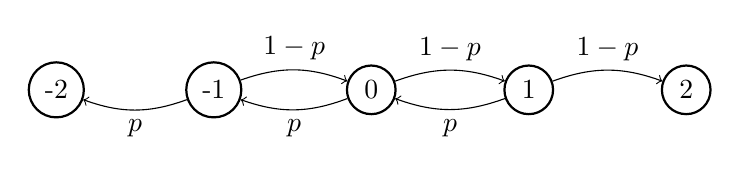
\begin{tikzpicture}
            \begin{scope}[every node/.style={circle,thick,draw}]
                \node (a) at (-4,0) {-2};
                \node (b) at (-2,0) {-1};
                \node (c) at (0,0) {0};
                \node (d) at (2,0) {1};
                \node (e) at (4,0) {2};
            \end{scope}
            \begin{scope}[every edge/.style={->,bend left=20,draw}]
                \path (b) edge node[midway,above]{$1-p$}(c);
                \path (c) edge node[midway,above]{$1-p$}(d);
                \path (d) edge node[midway,above]{$1-p$}(e);\path (d) edge node[midway,below]{$p$}(c);
                \path (c) edge node[midway,below]{$p$}(b);
                \path (b) edge node[midway,below]{$p$}(a);
            \end{scope}
        \end{tikzpicture}
    \end{center}

To prevent this, some sites try to obfuscate information, for example, you can only see a certain number of votes (the vote before you).

\begin{aexample}{Experts}{}
    For a given agent, there is probability $1-\epsilon$ of him being normal. A normal person has observation of inaccuracy $p\leq 1/2$. An expert gets a signal of probability $1$. Each agent knows their type but do not know what other's type are.
\end{aexample}

Under these assumptions, the first agent bids his signal. 
WLOG suppose the first agent got a high signal and bids `y'. If the second agent gets the same signal they will bid `y'. If the second agent is an expert they bid their own signal. So we suppose the second agent is normal and gets a low signal.
The odds that the item is good to bad is \[
    p*((1-\epsilon)*(1-p)+ \epsilon) : (1-p) *(1-\epsilon)*p = (1-\epsilon)*(1-p)+ \epsilon : (1-p)*(1-\epsilon) > 1:1
\]
This means that the second agent would follow the first bid! So every normal agent follows the first person. This happens until the first expert bids against the flow.

We can also add in crazy agents (uninformed) that bid randomly. If there are only crazy and normal people, the normal people will trust their own bid more and it takes more people to start a cascade.